\section{Cartes d'activation}

\subsection{Interpr\'etation des cartes d'activation de la premi\`ere couche}
Pour une image d'entr\'ee $X$ et une couche convolutionnelle $l$, la carte d'activation du canal $m$ est la r\'eponse spatiale
\begin{equation}
A_m^{(l)}(X)=\phi\!\left(z^{(l)}_{:,:,m}(X)\right),
\end{equation}
c'est-\`a-dire la sortie du filtre $m$ apr\`es convolution et non-lin\'earit\'e. Il convient donc de distinguer les filtres appris $K^{(l)}_{u,v,c,m}$, qui constituent les poids adaptables du r\'eseau, des cartes d'activation, qui d\'ependent \`a la fois de ces poids et de l'image analys\'ee. Les couches successives composent ainsi une banque de filtres locaux et des transformations non lin\'eaires hi\'erarchiques, conform\'ement au cadre pr\'esent\'e dans le cours \cite{lecun_convolutional_networks,manzanera_classification_apprentissage,poly_chap4_classifml}.

La pr\'esente section r\'eutilise le mod\`ele profond r\'egularis\'e $M3/R3$ retenu aux Sections~6 et~7. Le run de r\'ef\'erence correspond \`a une architecture \`a trois \'etages convolutionnels entra\^in\'ee pendant $15$ epochs avec Adam sur le m\^eme split CIFAR-10 r\'eduit et la m\^eme standardisation image par image ; il atteint $53.70\%$ d'accuracy sur l'ensemble de test, pour une accuracy finale de validation de $53.80\%$ et un maximum de validation de $54.10\%$. Pour garantir une lecture stable, le rapport retient comme image principale un exemple de la classe \textit{truck}, correctement class\'e avec une confiance de $0.9933$.

La figure~\ref{fig:section8_first_layer} pr\'esente les $16$ cartes produites par la premi\`ere couche convolutionnelle \texttt{conv\_s1\_1}, de taille $32\times 32\times 16$. Plusieurs canaux r\'eagissent nettement aux transitions de luminance entre la carrosserie du camion, l'horizon et la chauss\'ee, tandis que d'autres soulignent davantage les contrastes chromatiques entre le ciel bleu, les zones gris-beige du v\'ehicule et l'arri\`ere-plan. Une mesure objective fond\'ee sur des corr\'elations avec des proxys simples confirme cette lecture prudente : les canaux $1$, $14$ et $12$ sont les plus corr\'el\'es \`a la norme du gradient, tandis que les canaux $10$, $7$ et $8$ sont les plus sensibles au contraste chromatique. La moyenne du taux d'activations positives vaut $0.464$ et l'entropie spatiale normalis\'ee moyenne $0.847$, ce qui indique des cartes encore denses et localement interpr\'etables, coh\'erentes avec un premier niveau de d\'etection de contours, de contraste local et de motifs simples.

\begin{figure}[htbp]
\centering
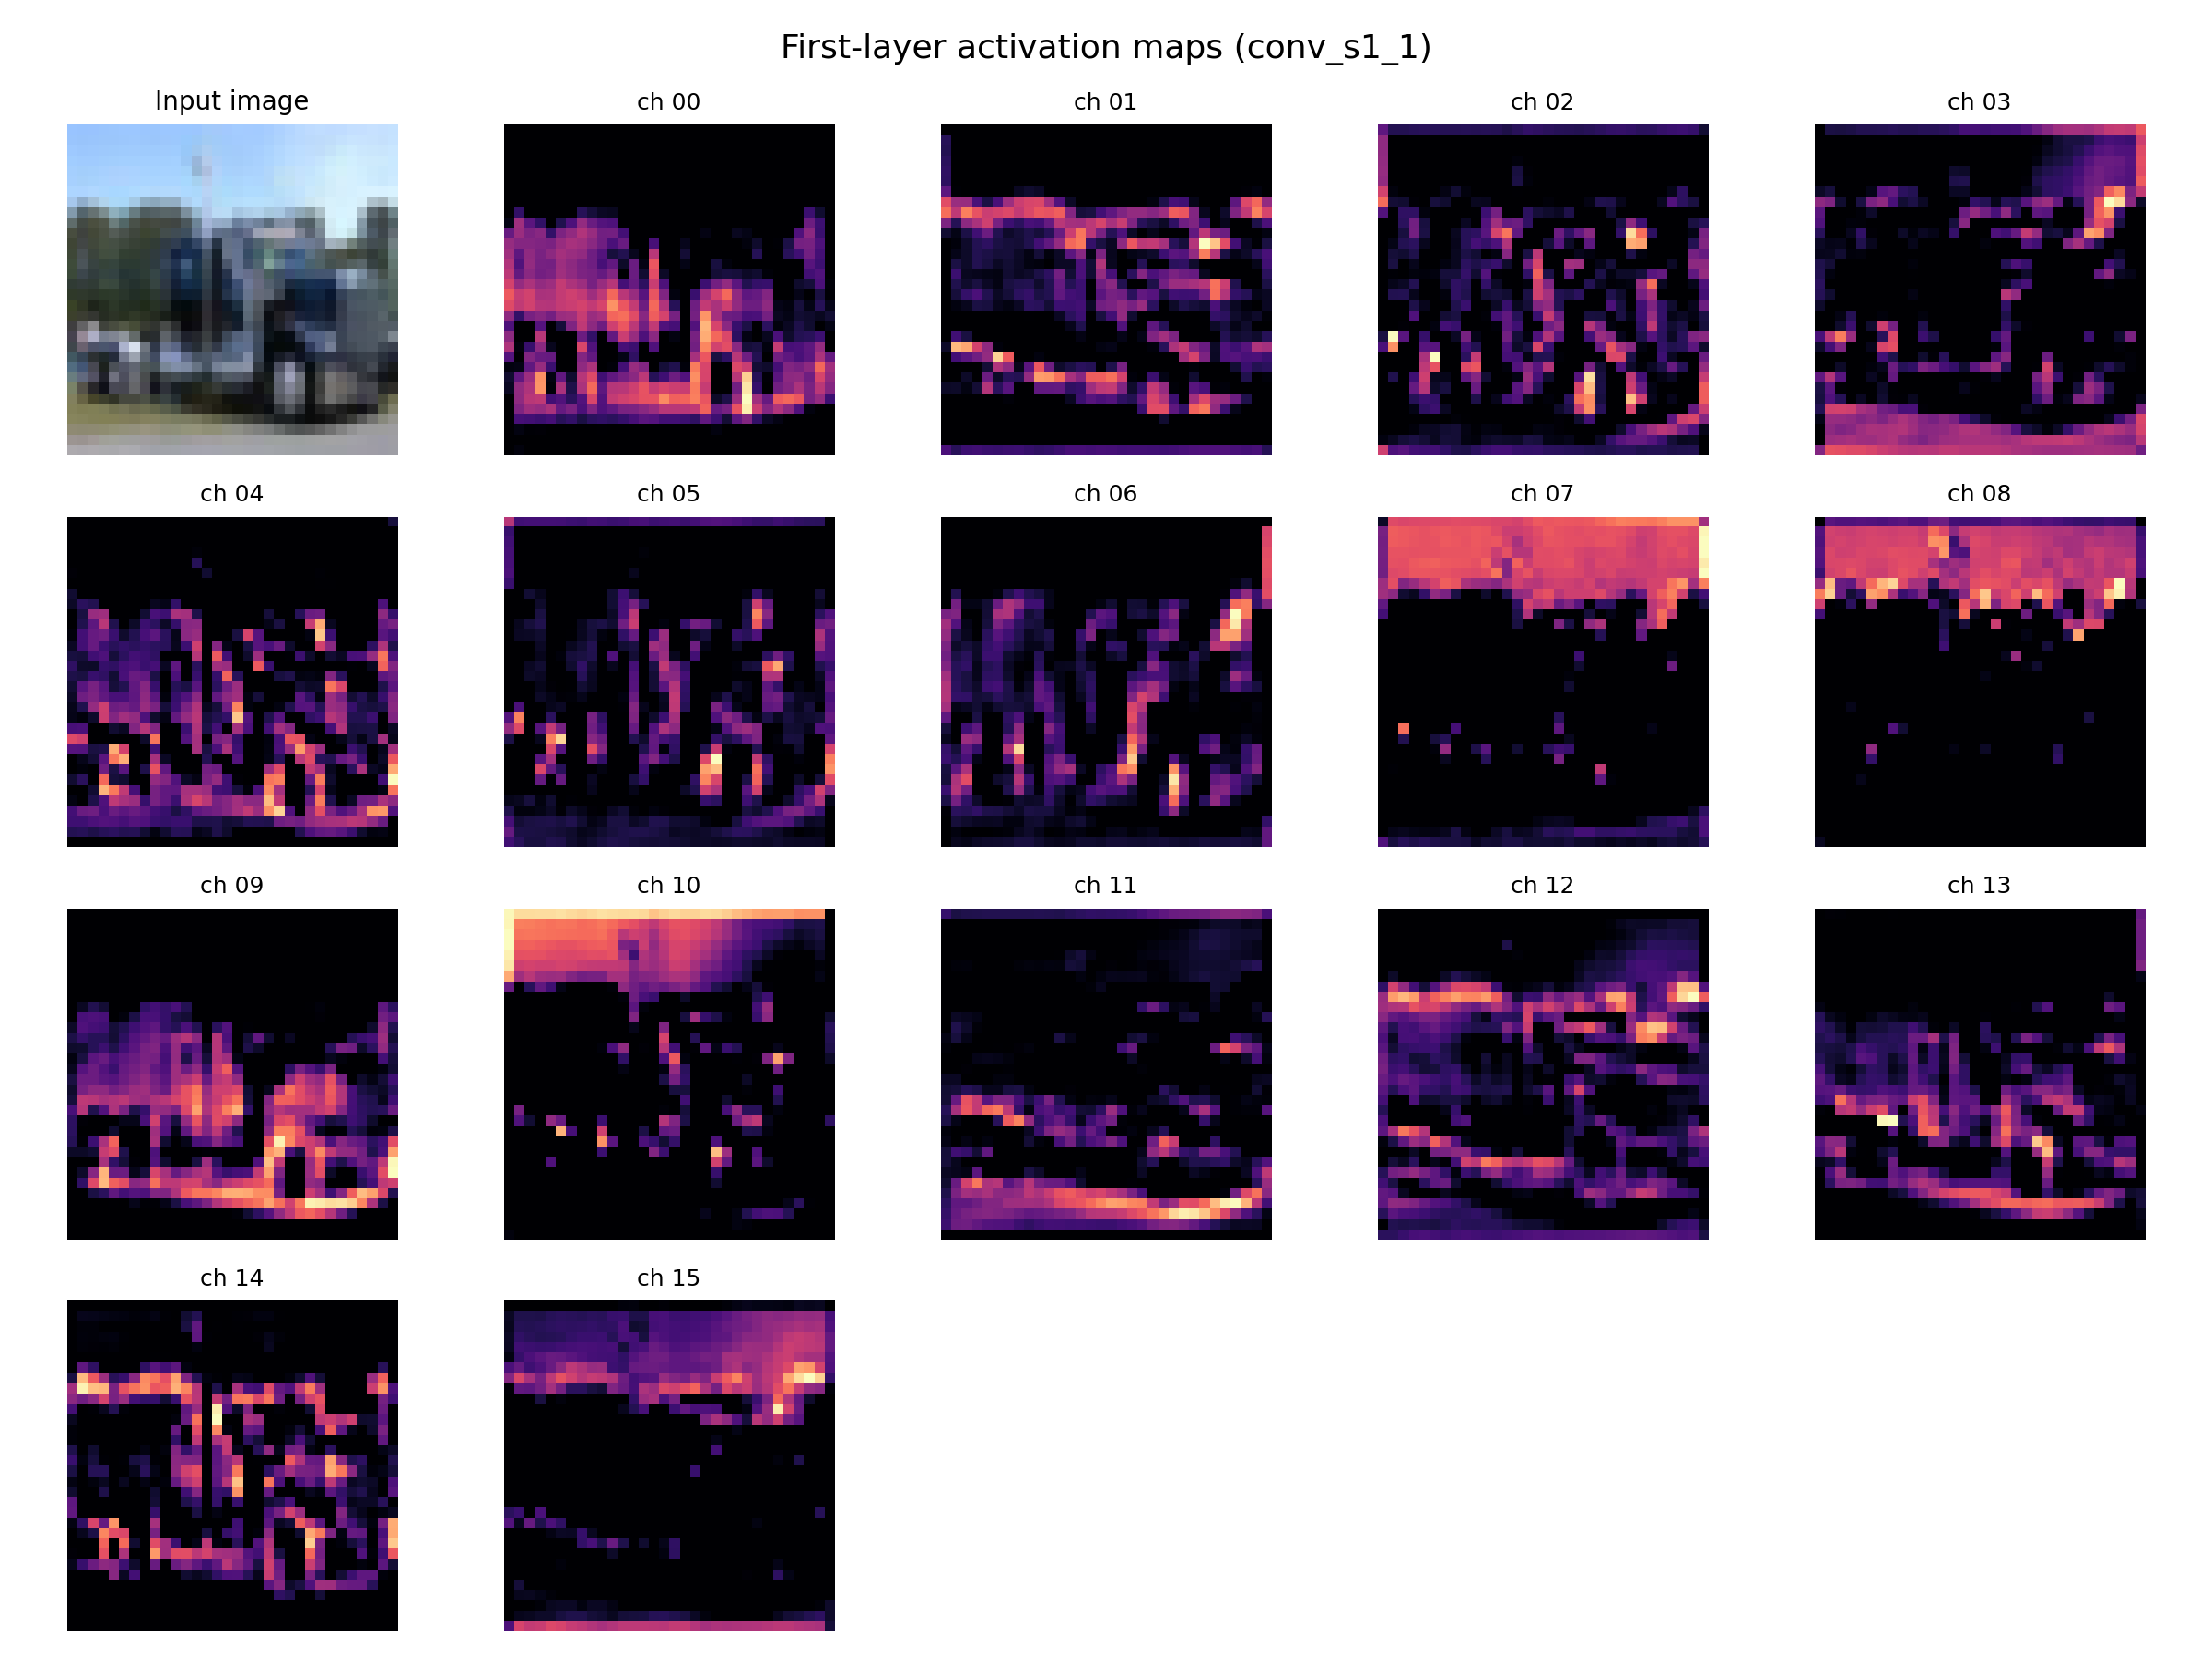
\includegraphics[width=0.5\textwidth]{imgs/section8_first_layer_activation_maps.png}
\caption{Cartes d'activation de la premi\`ere couche \texttt{conv\_s1\_1} pour l'image principale de la classe \textit{truck}. Le texte interne \`a la figure est laiss\'e en anglais pour garantir un rendu stable.}
\label{fig:section8_first_layer}
\end{figure}

\subsection{Cartes d'activation dans les couches profondes du mod\`ele raffin\'e}
L'analyse a ensuite port\'e sur les couches \texttt{conv\_s2\_2} et \texttt{conv\_s3\_2}, qui produisent respectivement des tenseurs de taille $16\times 16\times 32$ et $8\times 8\times 64$. La r\'eduction progressive de r\'esolution due aux op\'erations de \textit{pooling}, d\'ej\`a discut\'ee \`a la Section~6, augmente le champ r\'ecepteur effectif et conduit \`a des repr\'esentations moins directement lisibles \`a l'\'echelle du pixel. La figure~\ref{fig:section8_deep_layers} affiche, pour chaque couche, les $8$ canaux de plus forte activation moyenne sur la m\^eme image.

Par rapport \`a la premi\`ere couche, ces cartes apparaissent plus s\'electives et plus parcimonieuses. Le taux moyen d'activations positives passe de $0.422$ dans \texttt{conv\_s2\_2} \`a $0.402$ dans \texttt{conv\_s3\_2}, et l'entropie spatiale moyenne diminue de $0.780$ \`a $0.679$. Cette \'evolution est coh\'erente avec l'id\'ee d'une extraction hi\'erarchique : certaines cartes interm\'ediaires restent sensibles \`a des structures g\'eom\'etriques larges, alors que plusieurs cartes profondes se concentrent davantage sur des zones compatibles avec la silhouette du camion, ses roues ou l'opposition entre l'objet et l'arri\`ere-plan. Une interpr\'etation s\'emantique directe de chaque canal resterait toutefois excessive, car ces cartes repr\'esentent avant tout des r\'eponses internes utiles \`a la d\'ecision de classification.

\begin{figure}[htbp]
\centering
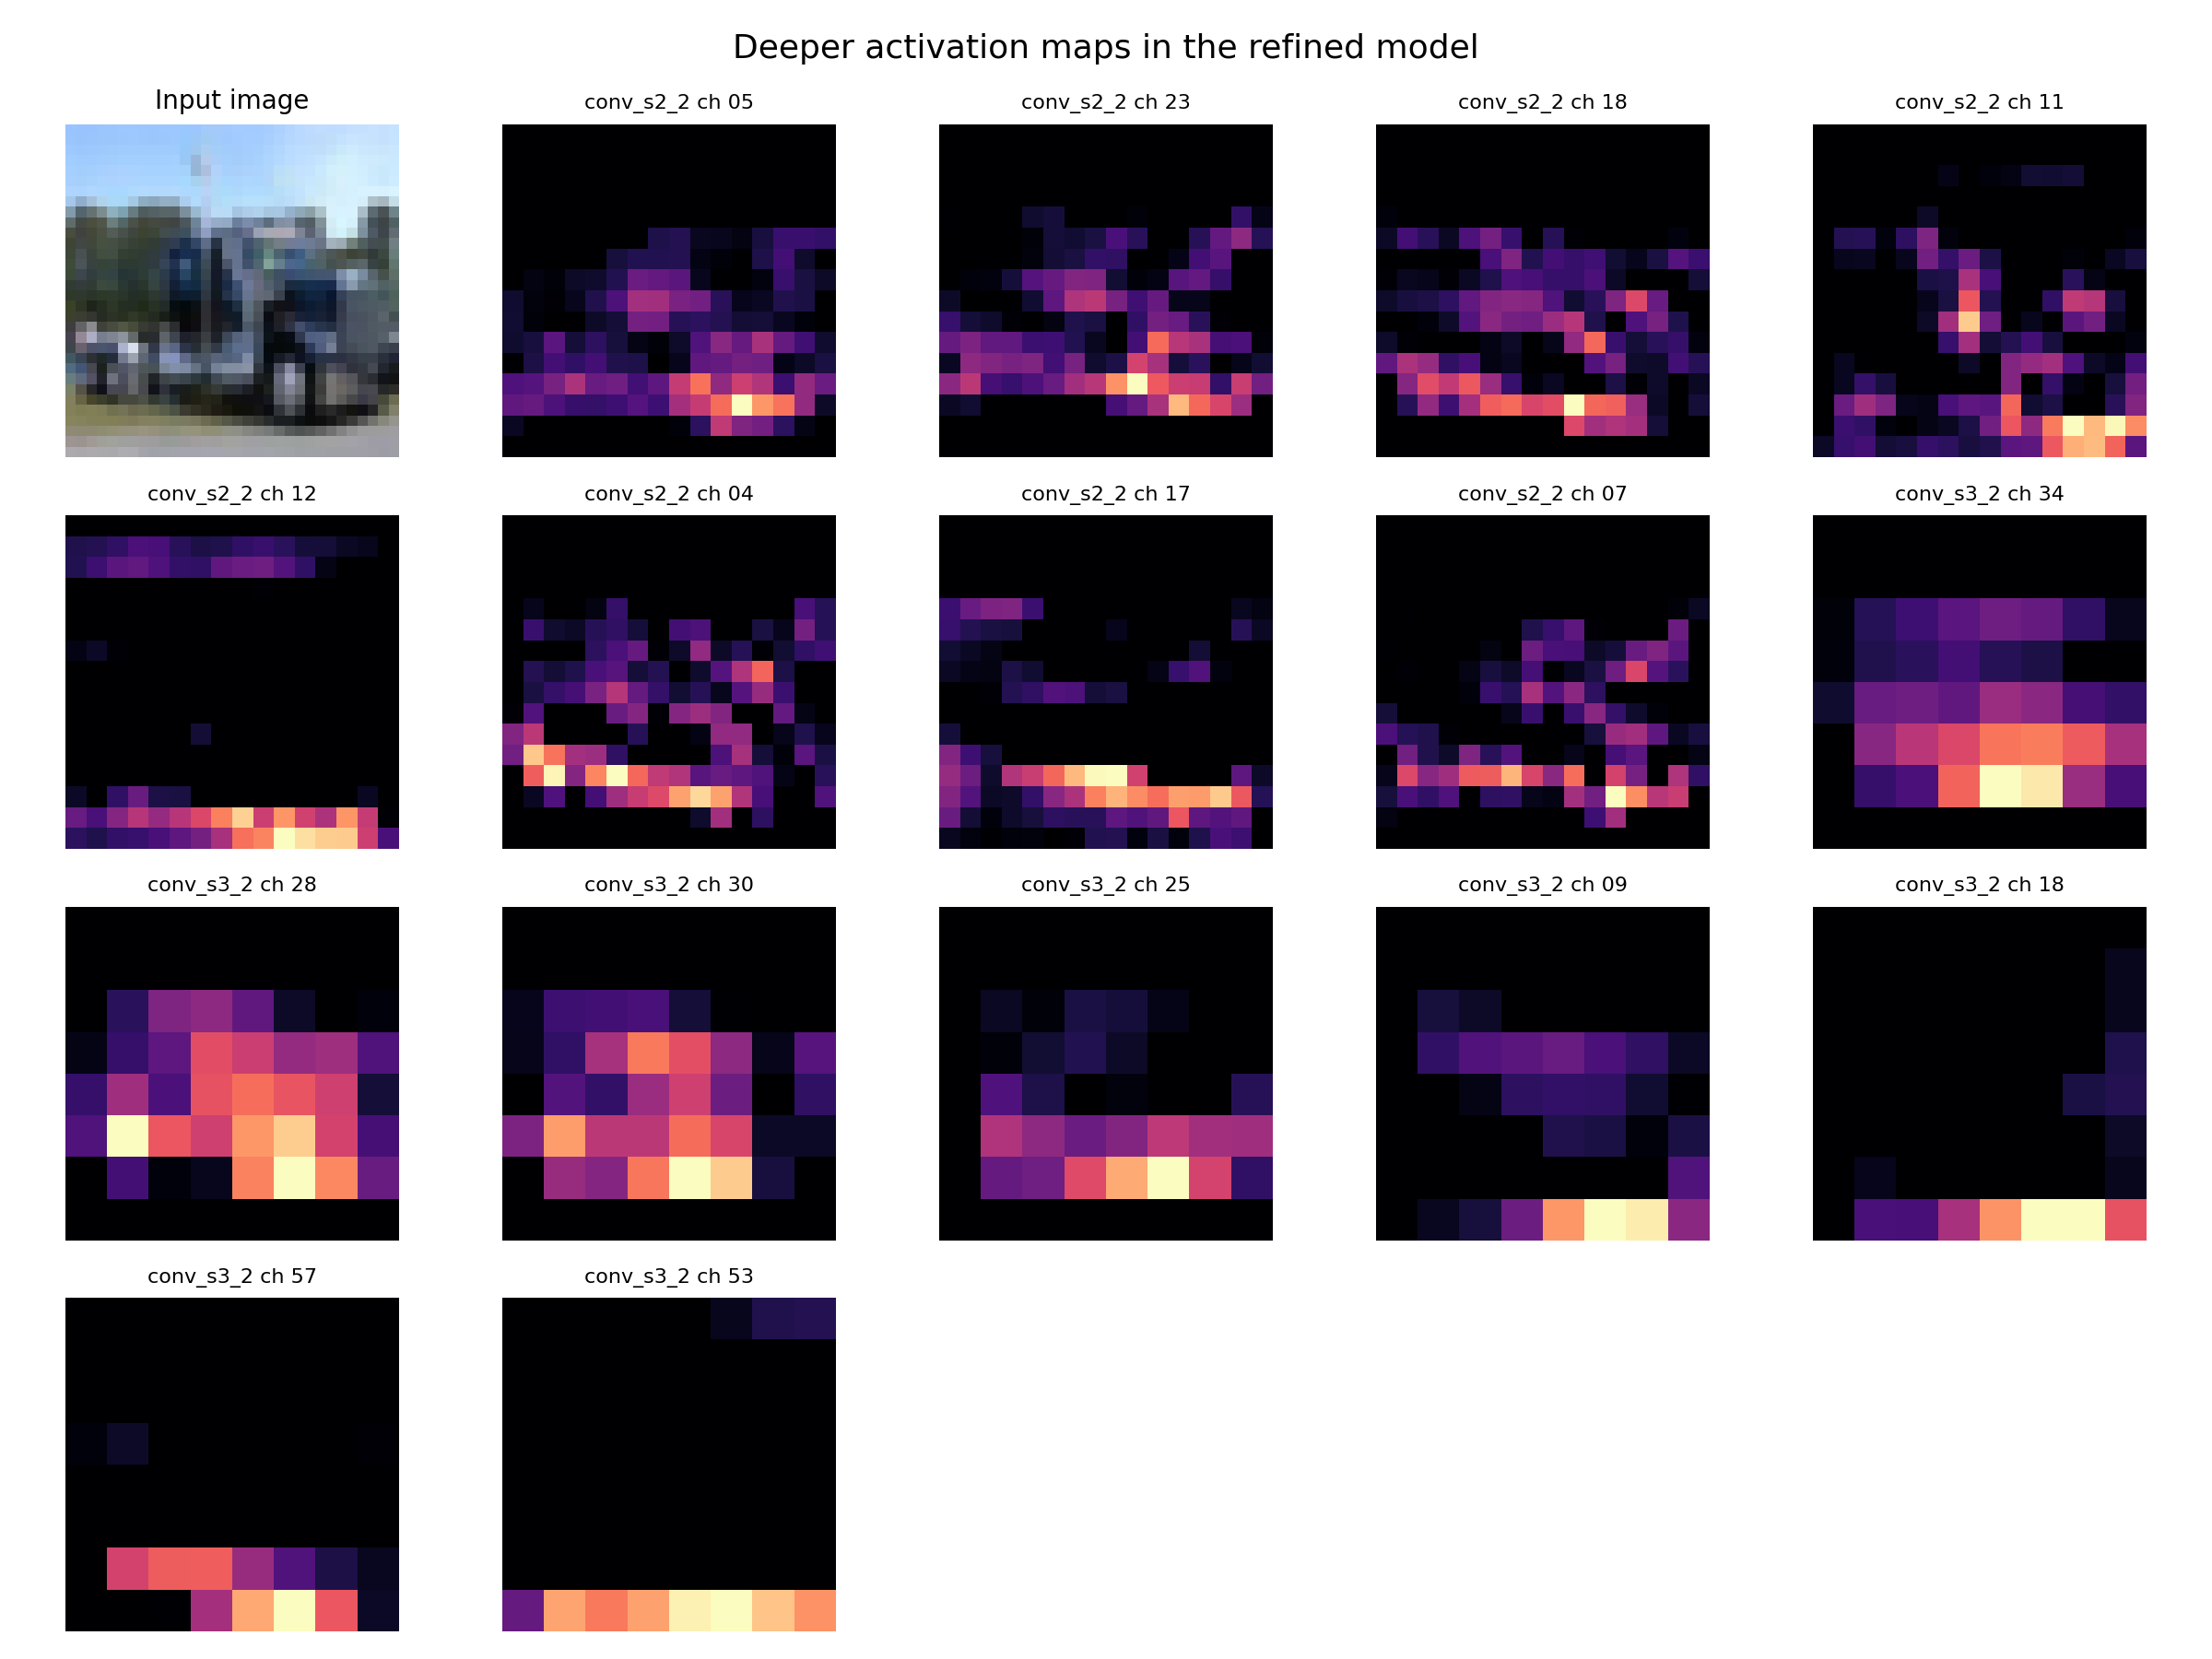
\includegraphics[width=0.5\textwidth]{imgs/section8_deep_layer_activation_maps.png}
\caption{Cartes d'activation de couches profondes du mod\`ele raffin\'e : top-$8$ de \texttt{conv\_s2\_2} et top-$8$ de \texttt{conv\_s3\_2}, class\'es par activation moyenne sur l'image principale.}
\label{fig:section8_deep_layers}
\end{figure}

\subsection{\'Evolution des cartes d'activation pendant l'apprentissage}
Aucun checkpoint exploitable n'\'etait disponible pour le mod\`ele profond final avant cette section ; un run de r\'ef\'erence a donc \'et\'e relanc\'e en sauvegardant uniquement les poids aux epochs $0$, $1$, $5$ et $15$. La comparaison a \'et\'e conduite sur la m\^eme image principale, avec les m\^emes canaux suivis \`a toutes les \'etapes : les canaux $12$ et $6$ de \texttt{conv\_s1\_1}, puis les canaux $34$ et $28$ de \texttt{conv\_s3\_2}, choisis \`a partir du mod\`ele final.

La figure~\ref{fig:section8_evolution} montre qu'\`a l'epoch $0$, avant toute mise \`a jour, les r\'eponses restent diffuses et peu structur\'ees. D\`es l'epoch $1$, certains contrastes spatiaux deviennent visibles, mais les cartes profondes conservent encore une organisation instable. \`A l'epoch $5$, les structures principales se stabilisent, et \`a l'epoch $15$ les cartes profondes apparaissent nettement plus localis\'ees sur des r\'egions discriminantes. Cette structuration progressive se retrouve dans des statistiques simples : l'\'ecart-type moyen des activations suivies n'augmente que de $0.031$ dans \texttt{conv\_s1\_1} entre les epochs $0$ et $15$, contre $0.303$ dans \texttt{conv\_s3\_2}. L'\'evolution des couches profondes est donc plus marqu\'ee que celle de la premi\`ere couche, ce qui sugg\`ere une sp\'ecialisation croissante des repr\'esentations internes au cours de l'apprentissage.

\begin{figure}[htbp]
\centering
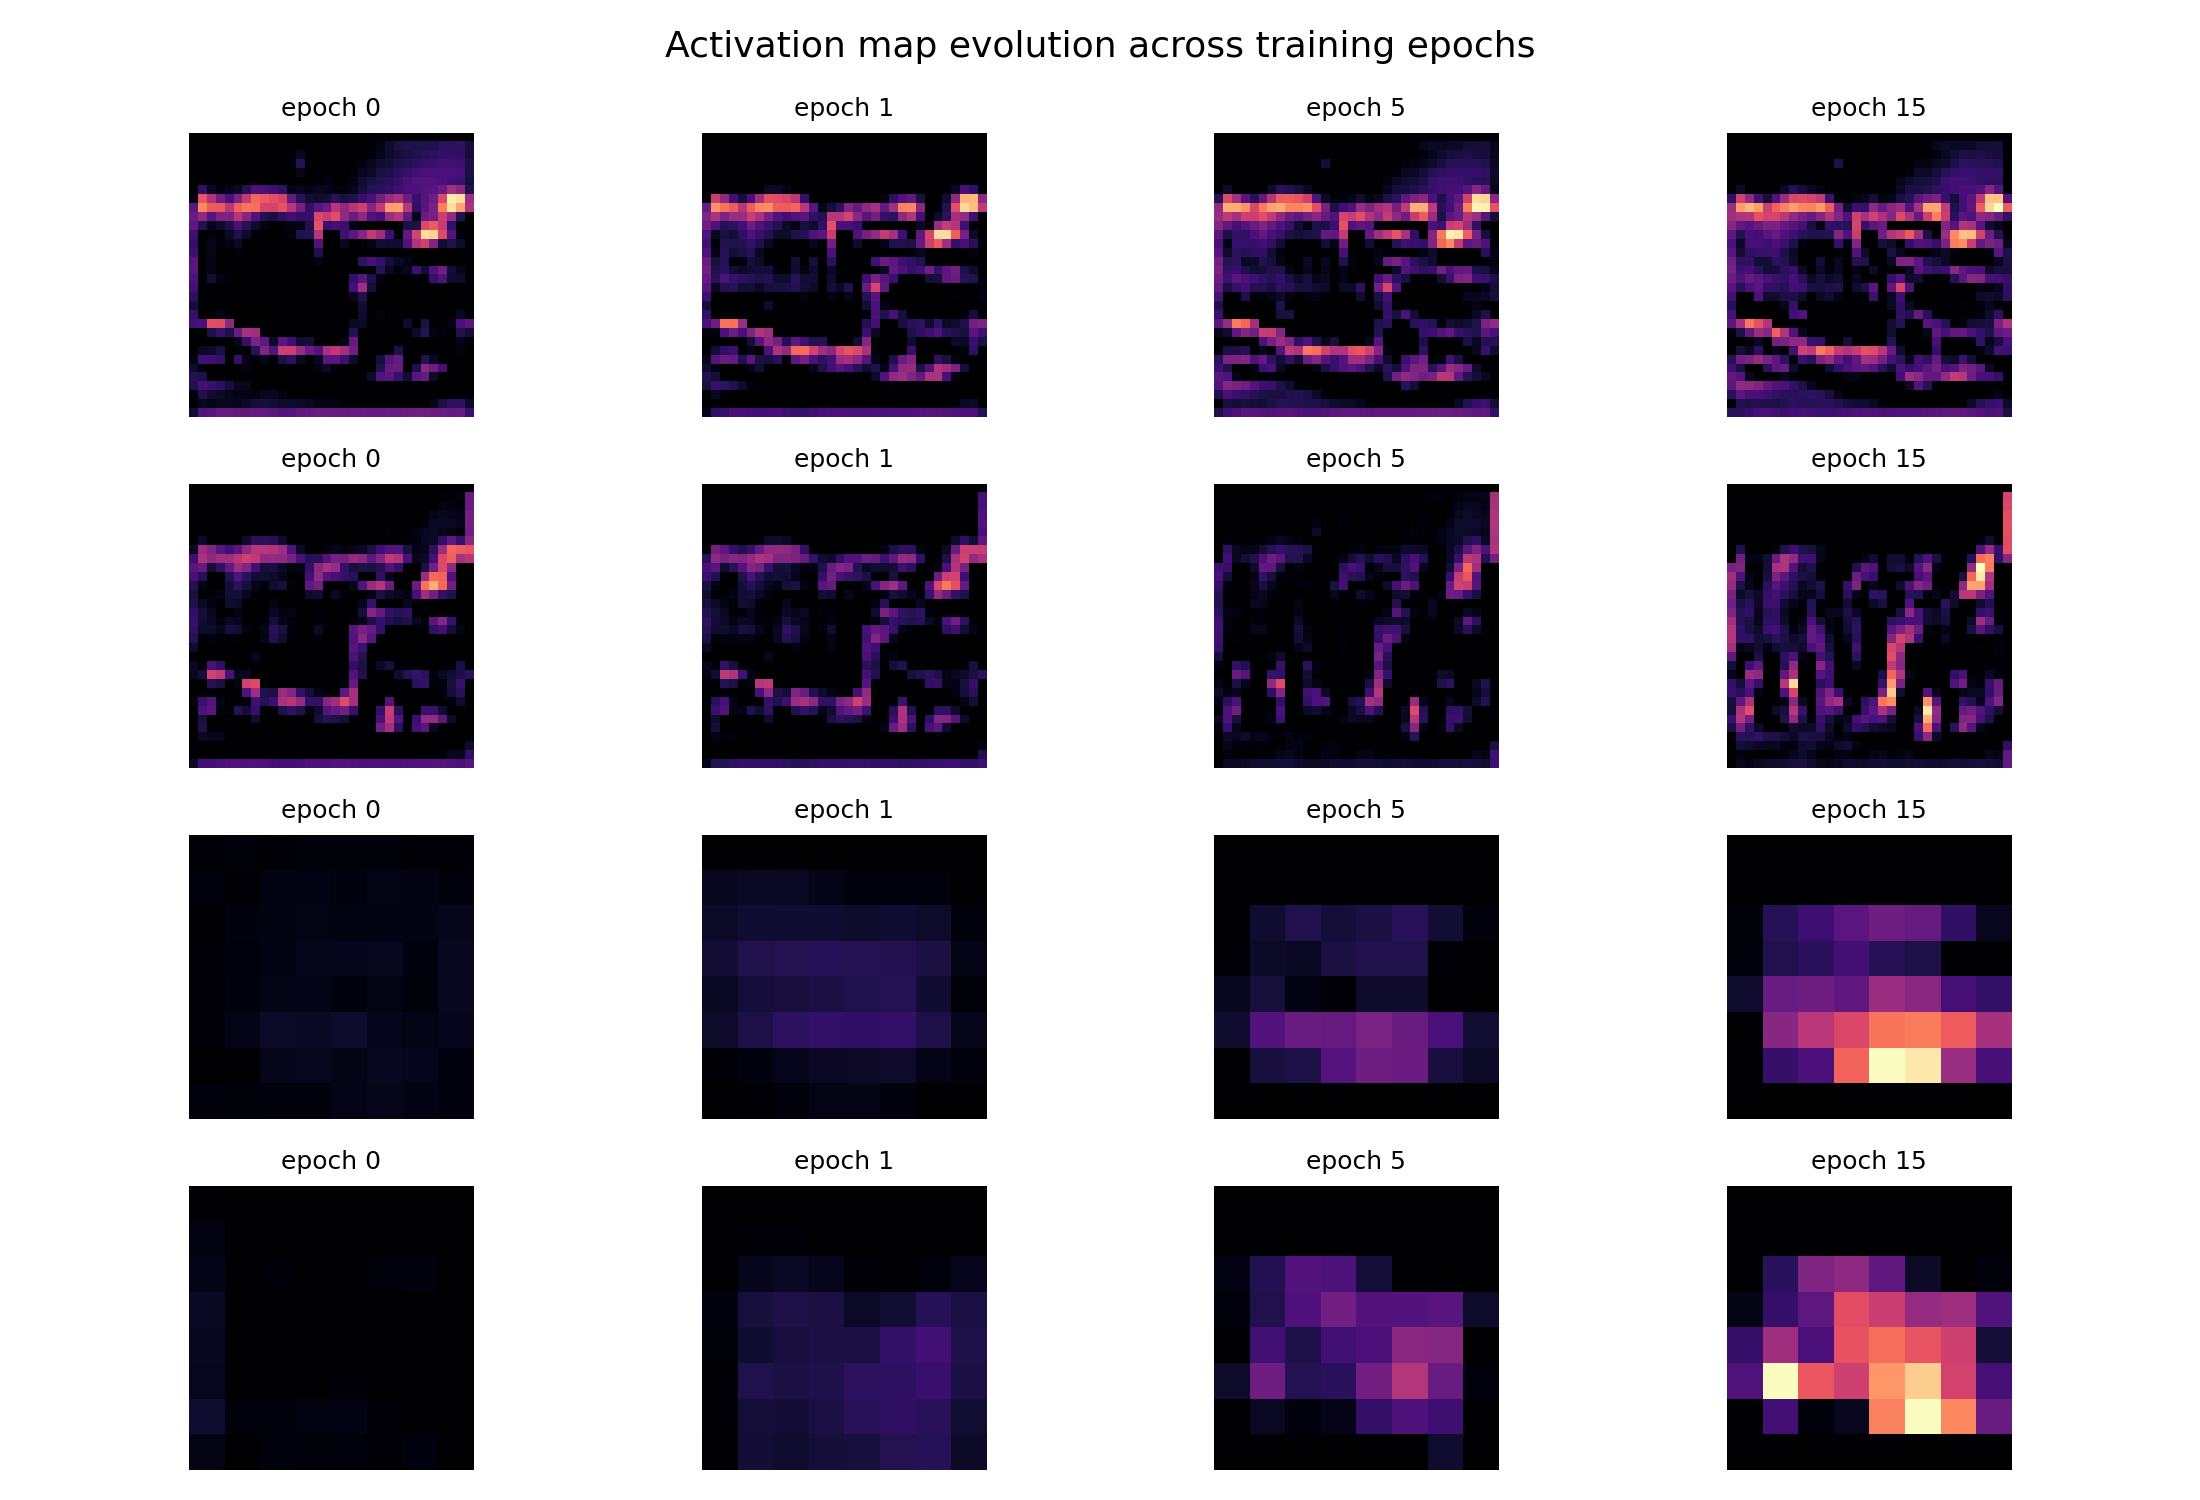
\includegraphics[width=0.5\textwidth]{imgs/section8_activation_evolution.png}
\caption{\'Evolution des cartes d'activation pour des canaux fix\'es de \texttt{conv\_s1\_1} et \texttt{conv\_s3\_2} aux epochs $0$, $1$, $5$ et $15$. La normalisation est fix\'ee par canal sur l'ensemble des epochs afin de rendre la comparaison temporelle lisible.}
\label{fig:section8_evolution}
\end{figure}

\begin{table*}[htbp]
\centering
\caption{Synth\`ese des visualisations retenues pour l'analyse des cartes d'activation.}
\label{tab:section8_summary}
\footnotesize
\begin{tabular}{|p{2.2cm}|p{2.7cm}|p{2.2cm}|p{1.4cm}|p{6.7cm}|}
\hline
Analyse & Couches inspect\'ees & Image retenue & Epochs & Observation concise \\
\hline
Premi\`ere couche & \texttt{conv\_s1\_1} & \textit{truck}, idx. $626$ & $15$ & $16$ cartes encore denses et localement interpr\'etables ; plusieurs canaux soulignent bords et contrastes chromatiques. \\
\hline
Couches profondes & \texttt{conv\_s2\_2}, \texttt{conv\_s3\_2} & \textit{truck}, idx. $626$ & $15$ & Top-$8$ par couche ; activations plus s\'electives et moins entropiques dans \texttt{conv\_s3\_2} que dans \texttt{conv\_s2\_2}. \\
\hline
\'Evolution temporelle & \texttt{conv\_s1\_1}, \texttt{conv\_s3\_2} & \textit{truck}, idx. $626$ & $0,1,5,15$ & M\^emes canaux suivis \`a toutes les \'etapes ; r\'eponses de plus en plus structur\'ees, surtout dans la couche profonde. \\
\hline
\end{tabular}
\end{table*}

\subsection{Discussion et limites d'interpr\'etation}
L'ensemble des visualisations reste coh\'erent avec les choix architecturaux des Sections~6 et~7. Les cartes de la premi\`ere couche traduisent des r\'eponses locales compatibles avec un banc de filtres sensibles aux bords, au contraste et \`a certaines oppositions chromatiques, tandis que les couches profondes deviennent plus s\'electives \`a mesure que le champ r\'ecepteur effectif s'accro\^it. L'\'evolution au cours des epochs montre en outre que les repr\'esentations profondes se structurent beaucoup plus fortement que les r\'eponses de bas niveau, ce qui est compatible avec l'apprentissage progressif de motifs utiles \`a la classification.

Ces cartes ne doivent toutefois pas \^etre sur-interpr\'et\'ees. Les figures reposent sur une normalisation min-max par carte pour les panneaux statiques, puis par canal sur l'ensemble des epochs pour la comparaison temporelle ; elles permettent donc une lecture qualitative, mais pas une comparaison absolue d'amplitude entre tous les canaux. Par ailleurs, une carte d'activation ne fournit pas \`a elle seule une causalit\'e directe sur la d\'ecision finale : elle renseigne sur des r\'eponses internes du r\'eseau, dont une partie seulement peut recevoir une interpr\'etation visuelle explicite. Enfin, le rapport se concentre volontairement sur une image principale pour conserver des figures lisibles ; l'inspection compl\'ementaire d'un exemple correctement class\'e de la classe \textit{frog} dans le notebook confirme les tendances g\'en\'erales, sans supprimer la part d'ambigu\"\i t\'e inh\'erente \`a ce type de visualisation.
